\begin{frame}
\frametitle{Outline}
\bi
\I Why do we need simulation methods for Bayesian inference?\vspace{2mm}
\I Sampling from posterior distributions using Markov chains\vspace{2mm}
\I Gibbs sampling\vspace{2mm}
\I Checking convergence of the MCMC simulations\vspace{2mm}
\I Checking efficiency of the MCMC simulations\vspace{2mm}
\I OpenBUGS demo
\ei

\end{frame}

\begin{frame}

\frametitle{Why is computation important?}

\bibig
\I Bayesian inference centres around the posterior distribution
   $$p(\btheta |y) \propto p(y|\btheta) \times p(\btheta)$$
   where $\btheta$ is typically a large vector of parameters
   $\btheta = \left\{\theta_1, \theta_2,....,\theta_k\right\}$\\ \vspace{2mm}
\I $p(y|\btheta)$ and $p(\btheta)$ will often be available in
   closed form, but $p(\btheta |y)$ is usually not analytically
   tractable, and we want to \\ \vspace{1mm}
   \nestedbi
   \I obtain marginal posterior $p(\theta_i |y)= \int\int...\int p(\btheta|y)\,\, d\btheta_{(-i)}$
      where $\btheta_{(-i)}$ denotes the vector of $\theta$s excluding $\theta_i$\\ \vspace{2mm}
   \I calculate properties of $p(\theta_i |y)$, such as mean
   $(=\int \theta_i p(\theta_i|y) d\theta_i)$, tail areas
   $(=\int_T^{\infty} p(\theta_i|y) d\theta_i)$ etc.\vspace{2mm}
   \nestedei
\I[$\rightarrow$] numerical integration becomes vital \eibig

\end{frame}

\begin{frame}

\frametitle{Monte Carlo integration}

\bi
\I We have already seen that Monte Carlo methods can be used to
simulate values from prior distributions and from \alert{closed form}
posterior distributions \\ \vspace{2mm}

\I If we had algorithms for sampling from arbitrary (typically
high-dimensional) posterior distributions, we could use Monte Carlo
methods for general Bayesian inference
\ei

\end{frame}

\begin{frame}

\frametitle{How do we sample from non-conjugate and high-dimensional posteriors?}

\bibig
\item We want samples from joint posterior distribution $p(\btheta | y)$\vspace{2mm}
\item \alert{Independent} sampling from $p(\btheta | y)$ may be difficult\vspace{2mm}
\item {\bf BUT} \alert{dependent} sampling from a \alert{Markov chain} with
   $p(\btheta | y)$ as its  stationary (equilibrium) distribution is easier \vspace{2mm}
\item A sequence of random variables
$\theta^{(0)},\theta^{(1)},\theta^{(2)},...$
   forms a Markov chain if $\theta^{(i+1)}  \sim  p(\theta | \theta^{(i)})$ \\ \vspace{1mm}
   \begin{itemize}
   \item[i.e.] conditional on the value of $\theta^{(i)} $,
   $\theta^{(i+1)}$ is independent of $\theta^{(i-1)},..., \theta^{(0)}$
   \end{itemize}
\eibig

\end{frame}

\begin{frame}

\frametitle{Sampling from the posterior using Markov chains}

Several standard \lq recipes' available for designing
      Markov chains with required stationary distribution $p(\btheta | y)$\vspace{2mm}
      \bibig
      \item Metropolis {\it et al.} (1953); generalised by Hastings (1970)\vspace{2mm}
      \item \alert{Gibbs Sampling} (see Geman and Geman (1984), Gelfand
           and Smith (1990), Casella and George (1992)) is a special case of
           the Metropolis-Hastings algorithm which  generates a
           Markov chain by sampling from \alert{full conditional distributions}\vspace{2mm}
      \item See Gilks, Richardson and  Spiegelhalter (1996) for a full
            introduction and many worked examples
\eibig

\end{frame}

\begin{frame}

\frametitle{Gibbs sampling}

Let our vector of unknowns $\btheta$ consist of $k$ sub-components
$\btheta = (\theta_1, \theta_2, \hdots , \theta_k)$ \\ \vspace{2mm}

\begin{itemize}
\item[1)] Choose starting values $\theta_1^{(0)},
\theta_2^{(0)}, \hdots , \theta_k^{(0)}$ \vspace{2mm}
\item[2)] Sample $\theta_1^{(1)}$ from $p(\theta_1 | \theta_2^{(0)}, \theta_3^{(0)},
\hdots , \theta_k^{(0)}, y)$ \vspace{1mm}
\item[] Sample $\theta_2^{(1)}$ from
$p(\theta_2 | \theta_1^{(1)}, \theta_3^{(0)}, \hdots , \theta_k^{(0)}, y)$ \vspace{1mm}
\item[] $\vdots$ \vspace{1mm}
\item[] Sample $\theta_k^{(1)}$ from $p(\theta_k |
\theta_1^{(1)}, \theta_2^{(1)}, \hdots , \theta_{k-1}^{(1)}, y)$\vspace{2mm}
\item[3)] Repeat step 2 many 1000s of times \vspace{1mm}
  \begin{itemize}
  \item eventually obtain sample from $p(\btheta | y)$\vspace{2mm}
  \end{itemize}
\end{itemize}

The conditional distributions are called \lq full conditionals' as they condition on all other parameters

\end{frame}

\begin{frame}[t]

\frametitle{Gibbs sampling continued}

Example with $k=2$

\vspace{-1.8cm}
\scalebox{0.7}{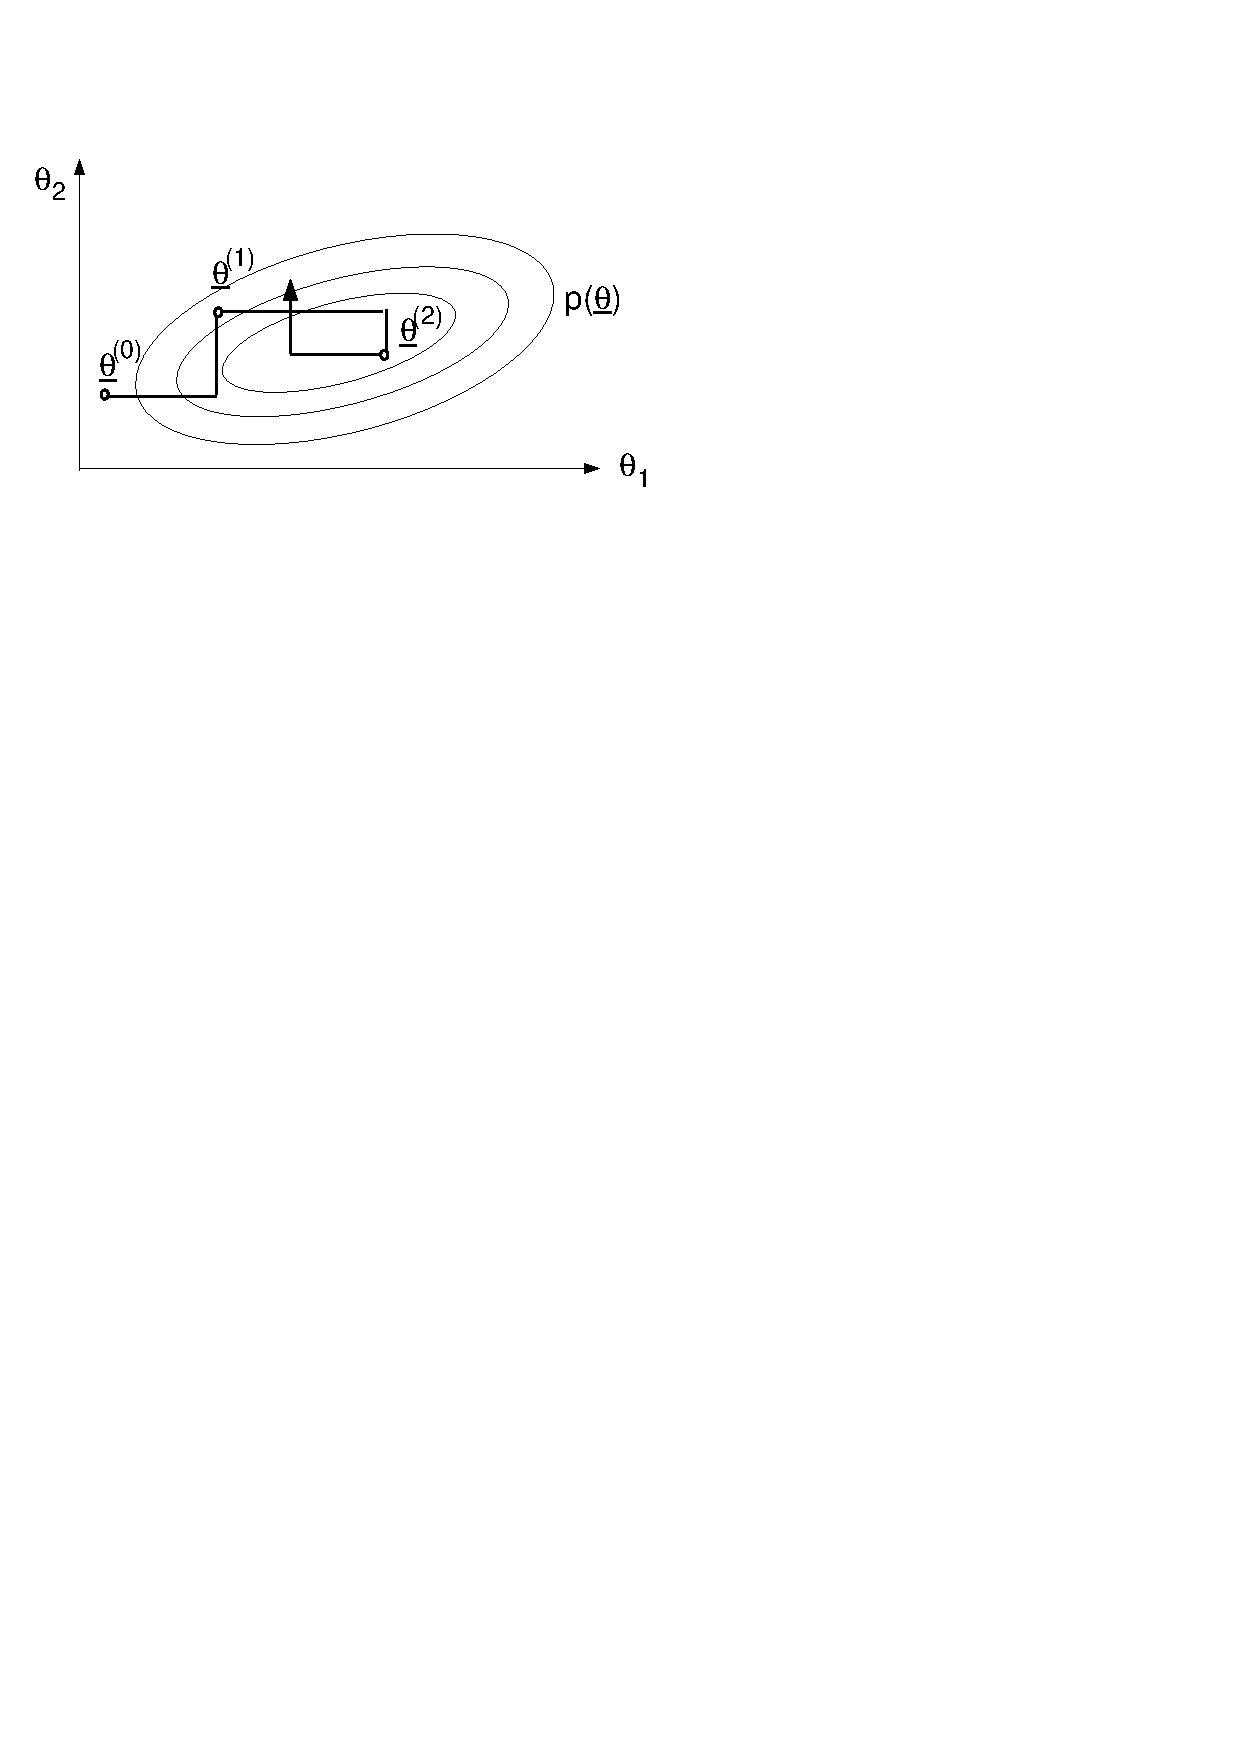
\includegraphics{Figures/gibbs.pdf}}
\vspace{-15.8cm}

\begin{itemize}
\item Sample  $\theta_1^{(1)}$ from   $p(\theta_1|\theta_2^{(0)}, y)$ \vspace{0.5mm}
\item Sample  $\theta_2^{(1)}$ from $p(\theta_2|\theta_1^{(1)}, y)$ \vspace{0.5mm}
\item Sample $\theta_1^{(2)}$ from $p(\theta_1|\theta_2^{(1)}, y)$ \vspace{0.5mm}
\item $\hdots$\vspace{1mm}
\end{itemize}
$\btheta^{(n)}$ forms a Markov chain with ({\em eventually}) a
 stationary distribution $p(\btheta | y)$

%%%%%%%%%%%%%%%%%%%%%%%%%%%%%%%%%%%%%%%%%%%%%%%%%%%%%%%%%%%%%%%%%%%
\end{frame}


 \begin{frame}[fragile]

\frametitle{Initial values}

\begin{itemize}
\item MCMC requires initial (starting) values to be specified for all unknown quantities\vspace{2mm}
\item OpenBUGS can automatically generate initial values using \emph{gen inits}\vspace{1mm}
      \bi
      \item these are generated from the prior distribution for each variable\vspace{2mm}
      \ei
\item OK if have informative priors\vspace{2mm}
\item  If have fairly \lq vague' priors, better for user to provide reasonable values in a separate initial values list\vspace{2mm}
\end{itemize}

Initial values list can be after model description or in a separate file, e.g.\vspace{-1mm}
\begin{verbatim}
list(theta=0.1)
\end{verbatim}\vspace{-1mm}
Note: initial values are just a starting point for the MCMC simulation, they are \alert{not} priors

\end{frame}


 \begin{frame}

 \frametitle{Using MCMC methods}

There are two main issues to consider\vspace{2mm}
\begin{enumerate}
\item Convergence\vspace{1mm}
  \bi
  \I how quickly does the distribution of
$\btheta^{(t)}$ approach $p(\btheta|y)$?\vspace{2mm}
  \ei
\item Efficiency\vspace{1mm}
  \bi
  \I how well are functionals of $p(\btheta|y)$ estimated from
$\{\btheta^{(t)}\}$?
  \ei
\end{enumerate}

\end{frame}

\begin{frame}[t]
\frametitle{Checking convergence}

This is the users responsibility!\vspace{2mm}

\bibig
\item Note: Convergence is to target \alert{distribution}
  (the required posterior), not to a single value\vspace{2mm}
\item Once convergence reached, samples should look like
  a random scatter about a stable mean value
\eibig

\end{frame}


\begin{frame}

\frametitle{Convergence diagnosis}

\bibig
\item How do we know we have reached convergence?\vspace{1mm}
    \bi
    \item i.e.~how do we know the number of \lq burn-in' iterations?\vspace{2mm}
    \ei
\item Many \lq convergence diagnostics' exist, but none foolproof\vspace{2mm}
\item CODA and BOA software contain large number of diagnostics\vspace{3mm}
\eibig

\alert{Brooks-Gelman-Rubin (bgr) diagnostic}\vspace{1mm}

\bibig
\item Multiple ($\ge 2$) runs\vspace{1mm}
\item Widely differing starting points\vspace{1mm}
\item Convergence assessed by quantifying whether sequences are much
further apart than expected based on their internal variability\vspace{1mm}
\item Diagnostic uses components of variance of the multiple sequences
\eibig

\end{frame}


\begin{frame}[t]

\frametitle{Example of checking convergence}

Consider the following response rates for different doses of a drug (similar to example from Practical 3 last week)

\begin{center}
\begin{tabular}{ccc}
dose $x_i$ & No. subjects $n_i$& No. responses $r_i$\\ \hline
1.69&59&6\\
1.72&60&13\\
1.75&62&18\\
1.78&56&28\\
1.81&63&52\\
1.83&59&53\\
1.86&62&61\\
1.88&60&60
\end{tabular}
\end{center}

Fit a logistic regression (uncentred analysis)
\begin{eqnarray*}
r_i & \sim & \hbox{Binomial}(p_i, n_i)\\
\hbox{logit } p_i & = & \alpha + \beta x_i\\
\alpha \; \sim \; {\rm N}(0, 10000) & &
\beta \; \sim\; {\rm N}(0, 10000)
\end{eqnarray*}

\end{frame}

\begin{frame}

\frametitle{Checking convergence with multiple runs}

\bibig
  \item Set up multiple initial value lists, e.g.\\ [2pt]
 \texttt{list(alpha=-100, beta=100)}\\
 \texttt{list(alpha=100, beta=-100)}\vspace{2mm}
  \item Before clicking \emph{compile}, set \emph{num of chains} to 2\vspace{2mm}
  \item Load both sets of initial values\vspace{2mm}
  \item Monitor from the start of sampling\vspace{2mm}
  \item Visually inspect trace/history plots to see if chains are
  overlapping\vspace{2mm}
  \item Assess how much burn-in needed using the \emph{bgr}
  statistic\vspace{2mm}
  \item Check autocorrelation, as high autocorrelation is symptom of
  slow convergence
\eibig

\end{frame}


\begin{frame}[t]

\begin{center}
\scalebox{0.45}{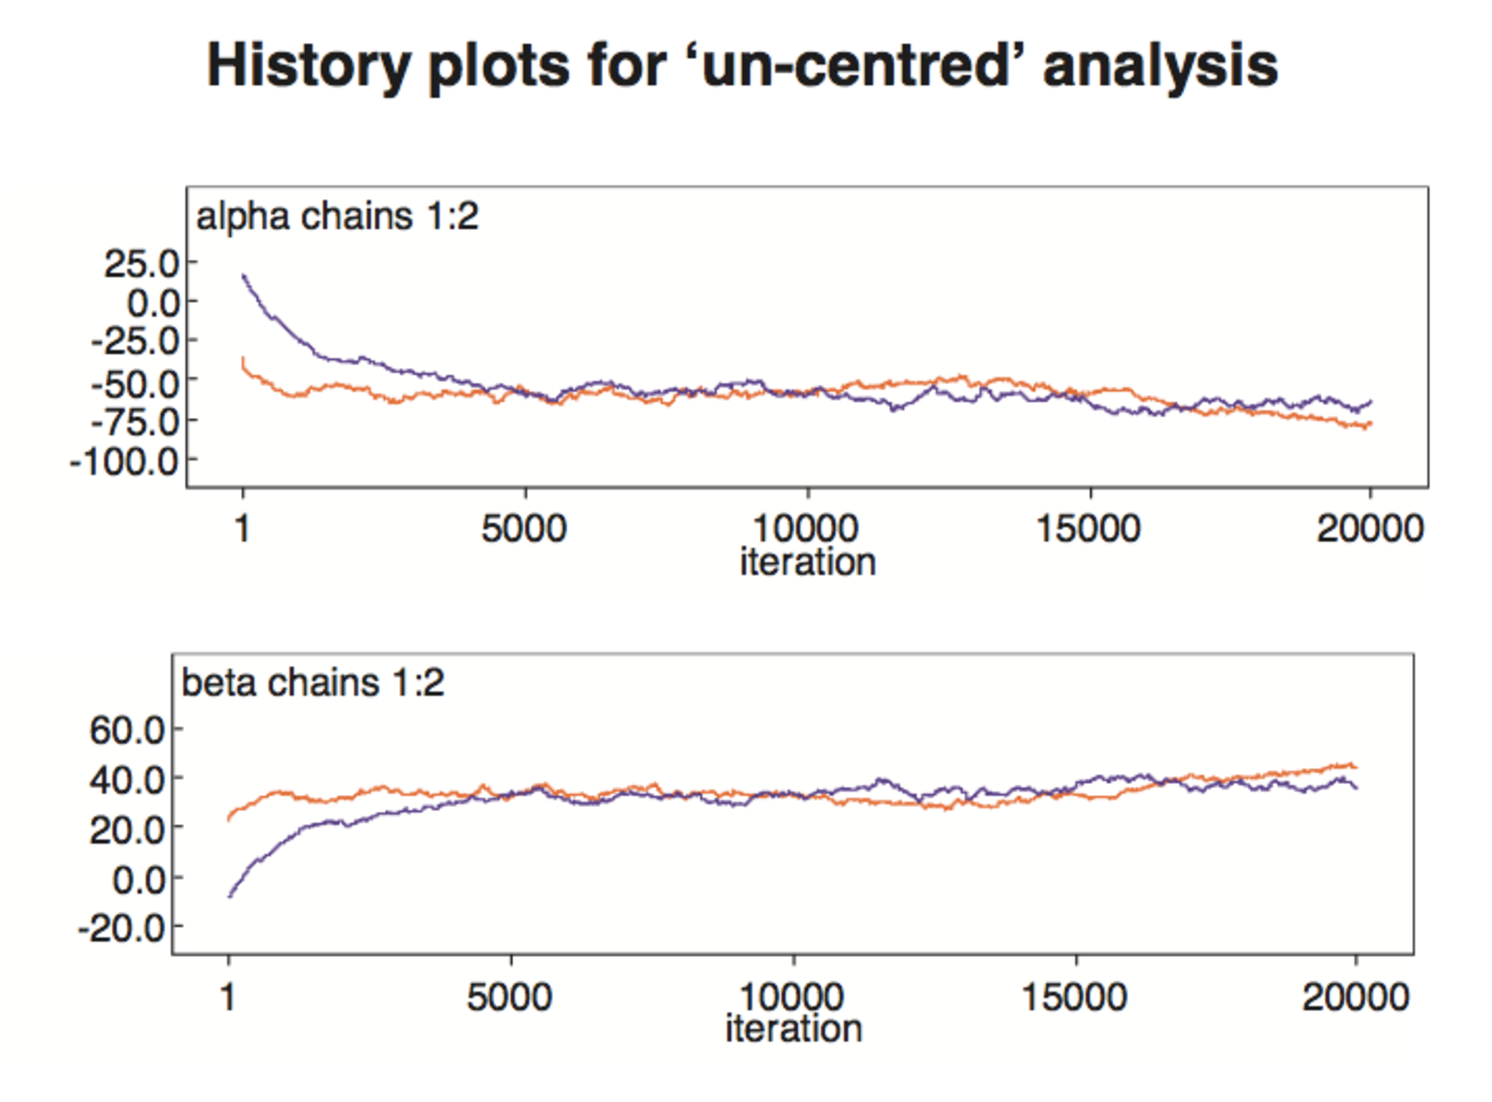
\includegraphics{Figures/dose-uncent-trace.pdf}}
\end{center}

\end{frame}


\begin{frame}[fragile,t]

\frametitle{bgr plot for uncentred analysis}
\begin{center}
\scalebox{0.4}{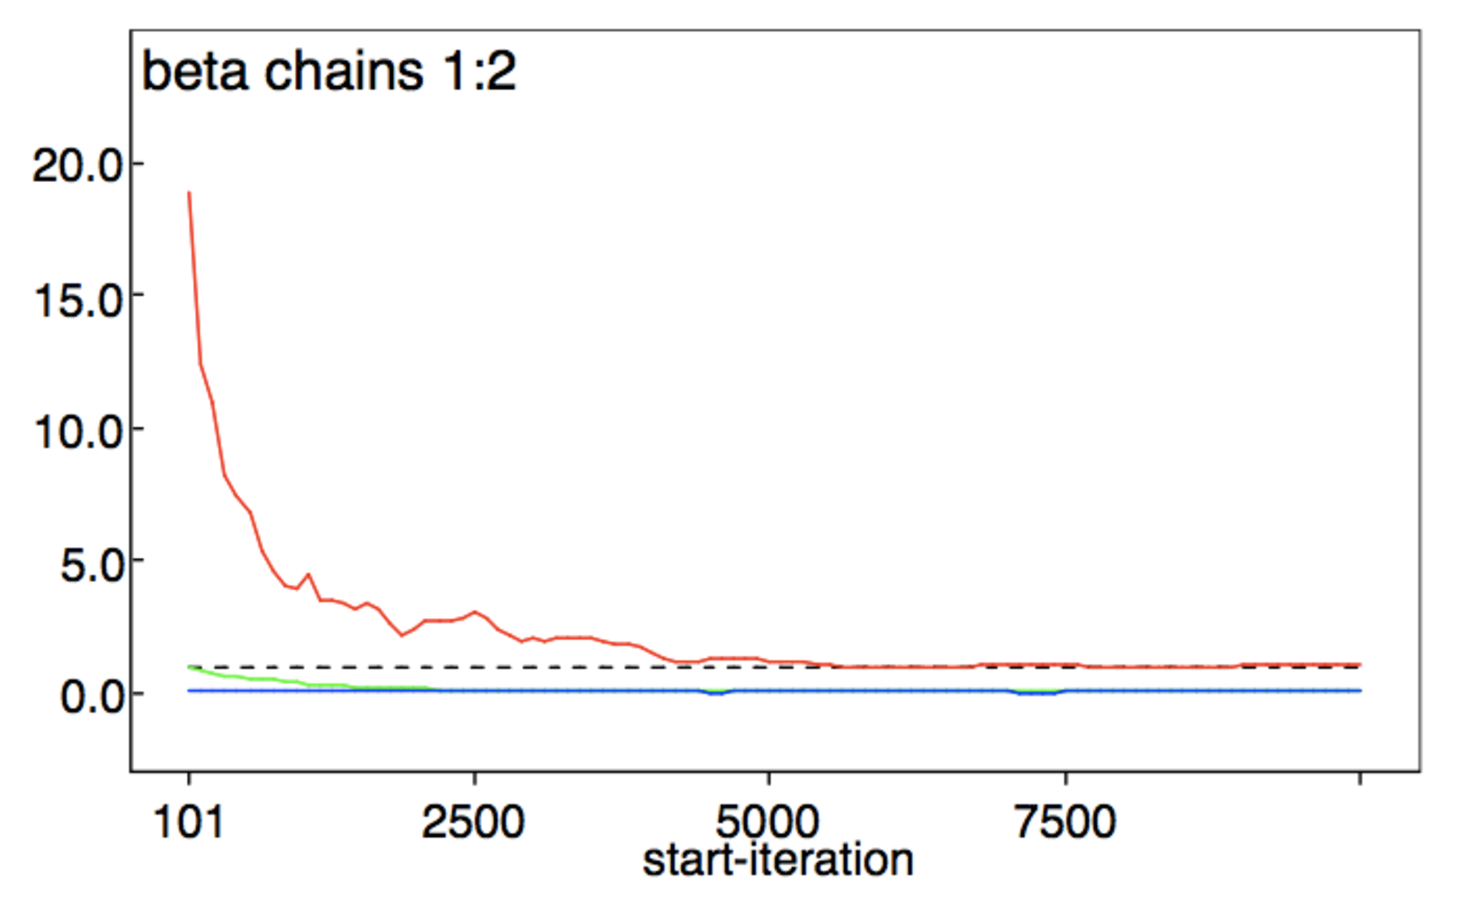
\includegraphics{Figures/dose-uncent-bgr-2009.pdf}}
\end{center}

Discard first 10,000 iterations as burn-in
\begin{footnotesize}
\begin{verbatim}
node  mean   sd    MC error 2.5%   median  97.5%  start sample
beta  33.36  3.00  0.2117   28.18  33.5    38.33  10001 20000
\end{verbatim}
\end{footnotesize}
\end{frame}


 \begin{frame}
\frametitle{BGR convergence diagnostic in OpenBUGS}

\begin{center}
\scalebox{0.38}{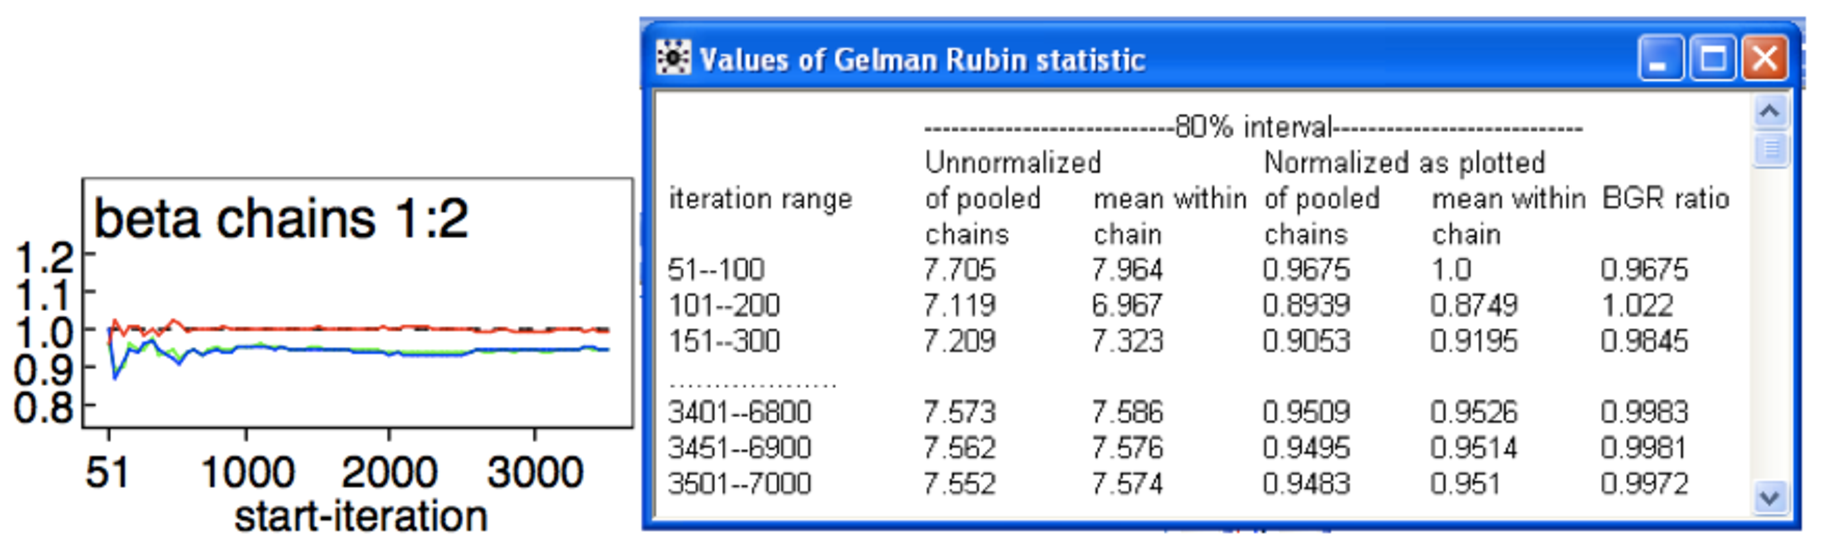
\includegraphics{Figures/bgr-plot-stats.pdf}}
\end{center}
\centerline{Interpreting the \emph{bgr} statistics}\vspace{2mm}
When convergence is reached:\vspace{2mm}
\bi
  \item \emph{Green}: width of 80\% intervals of pooled chains: should be stable\vspace{2mm}
  \item \emph{Blue}: average width of 80\% intervals for chains: should be stable\vspace{2mm}
  \item \emph{Red}: ratio of pooled/within: should be near 1\vspace{2mm}
\ei

\end{frame}


\begin{frame}

\frametitle{BGR convergence diagnostic in OpenBUGS}
\begin{center}
\scalebox{0.38}{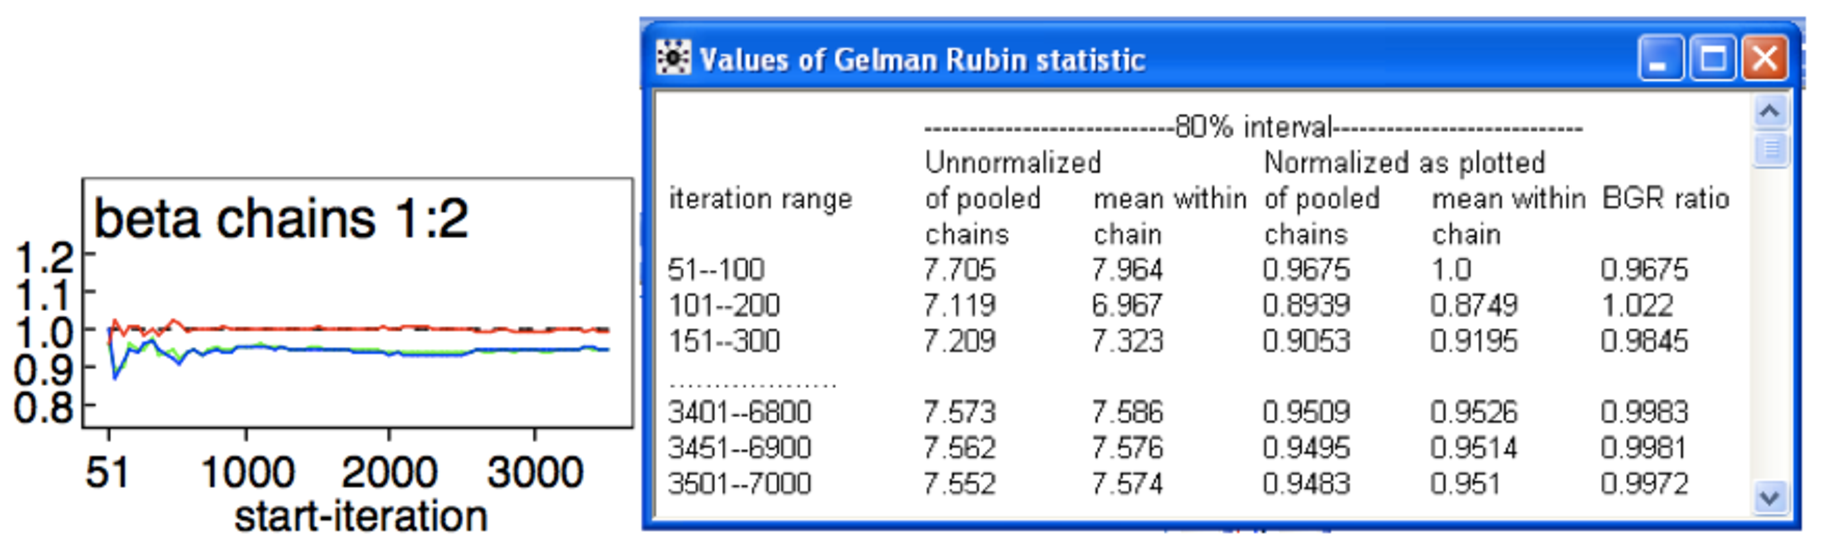
\includegraphics{Figures/bgr-plot-stats.pdf}}
\end{center}
 \bi
  \item OpenBUGS splits iterations into multiple overlapping
  intervals, calculates \emph{bgr} statistics for each interval,
  and plots them against starting iteration of interval\vspace{0.5mm}
  \bi
  \item approximate convergence can be \lq read off' plot as
  iteration after which  red \emph{bgr} ratio line stabilises
  around 1, and blue and green 80\% interval lines
  stabilise to approximately constant value (not necessarily 1)\vspace{1mm}
  \ei
  \item In OpenBUGS, right-click on the plot, select \emph{Properties}, then click on \emph{Data} gives values of statistics
\ei

\end{frame}


\begin{frame}[fragile]
\begin{center}
\scalebox{0.38}{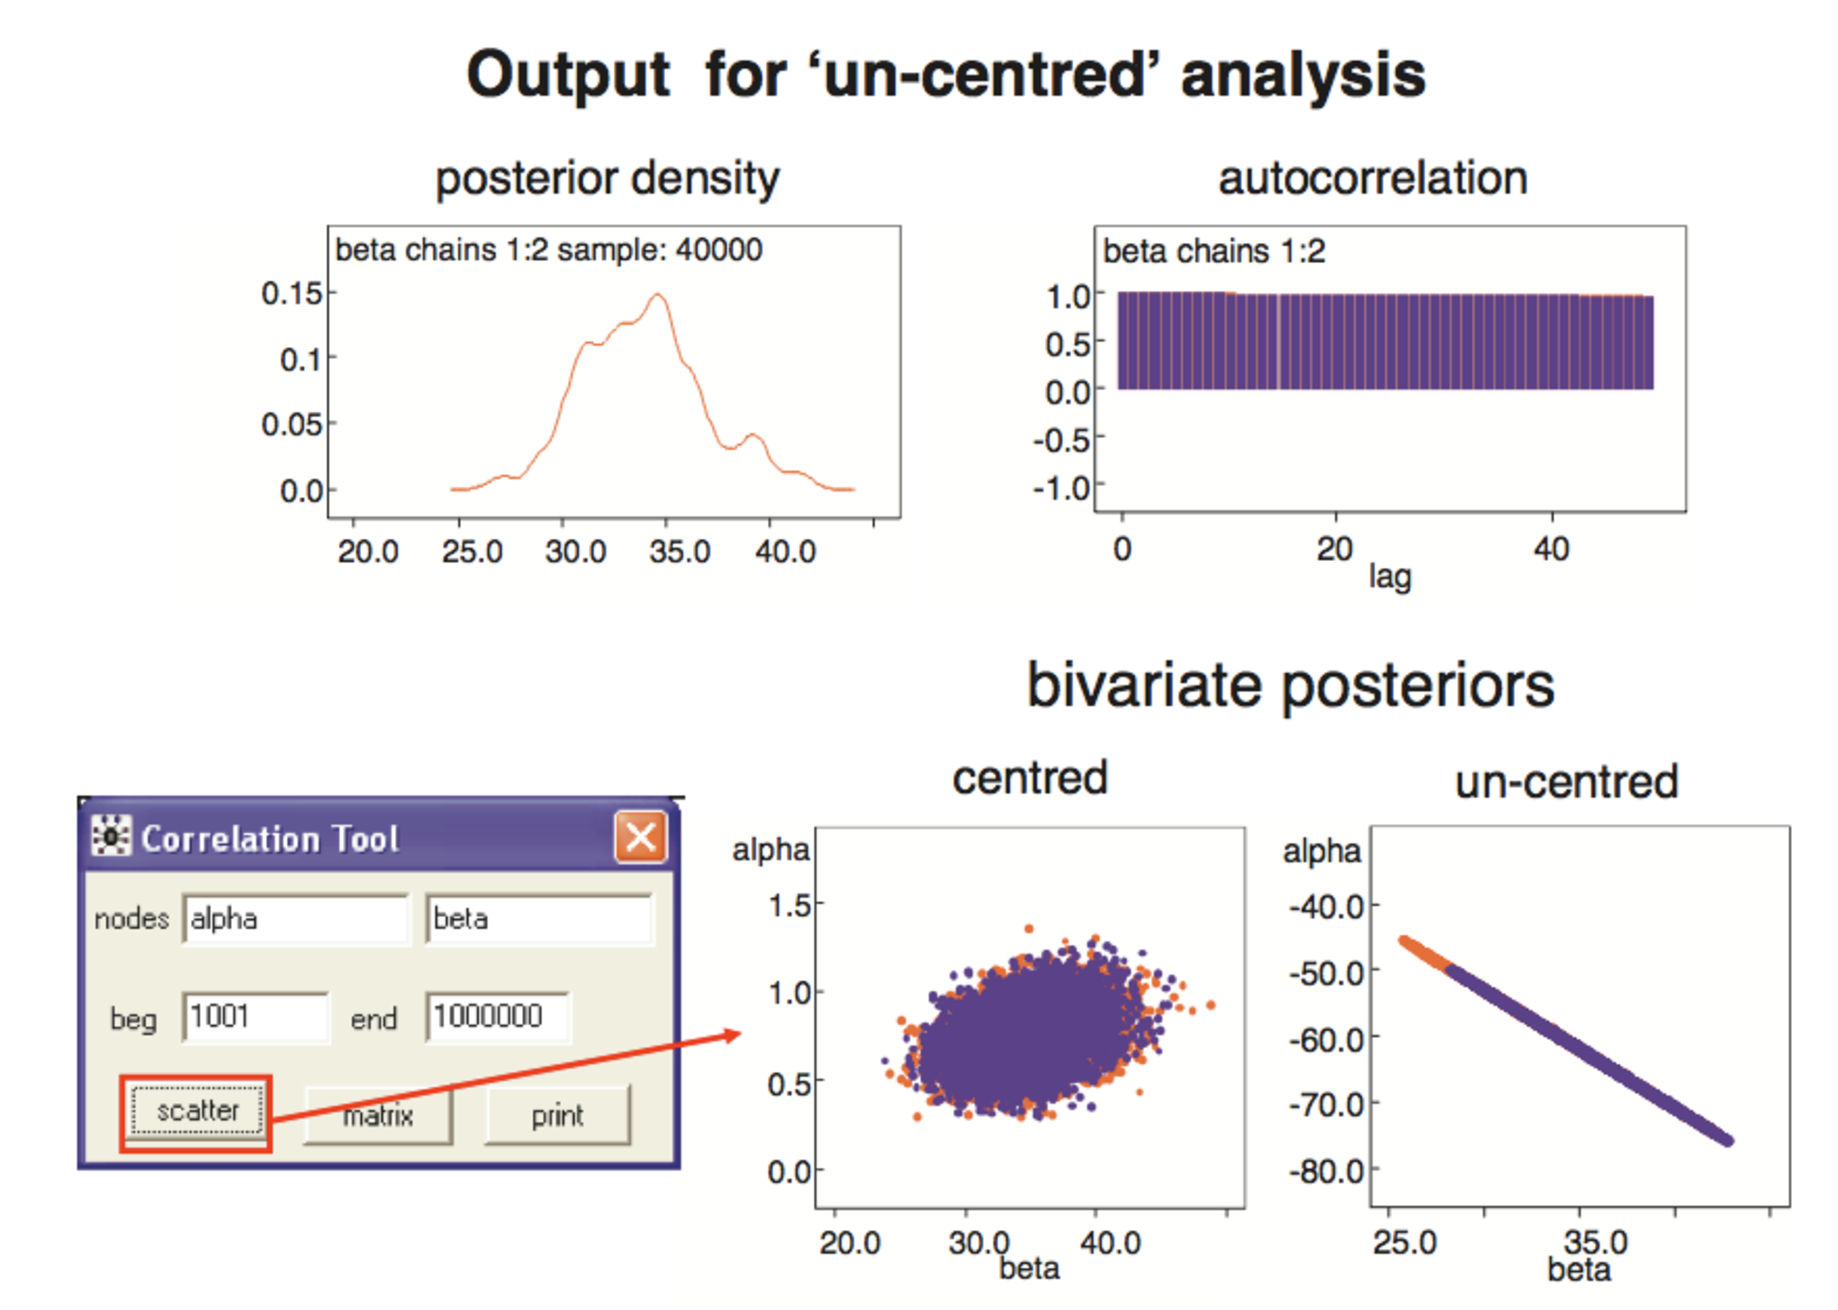
\includegraphics{Figures/dose-uncent-out.pdf}}
\end{center}
\end{frame}


\begin{frame}[fragile]
\vspace{2mm}Re-fit same logistic regression, but with centred covariate
\begin{eqnarray*}
r_i & \sim & \hbox{Binomial}(p_i, n_i)\\
\hbox{logit } p_i & = & \alpha^* + \beta (x_i - \bar{x})\\
\alpha^* & \sim &{\rm N}(0, 10000)\\
\beta & \sim& {\rm N}(0, 10000)
\end{eqnarray*}
Note: $\alpha^* = \alpha + \beta \bar{x}$
\begin{center}
\scalebox{0.38}{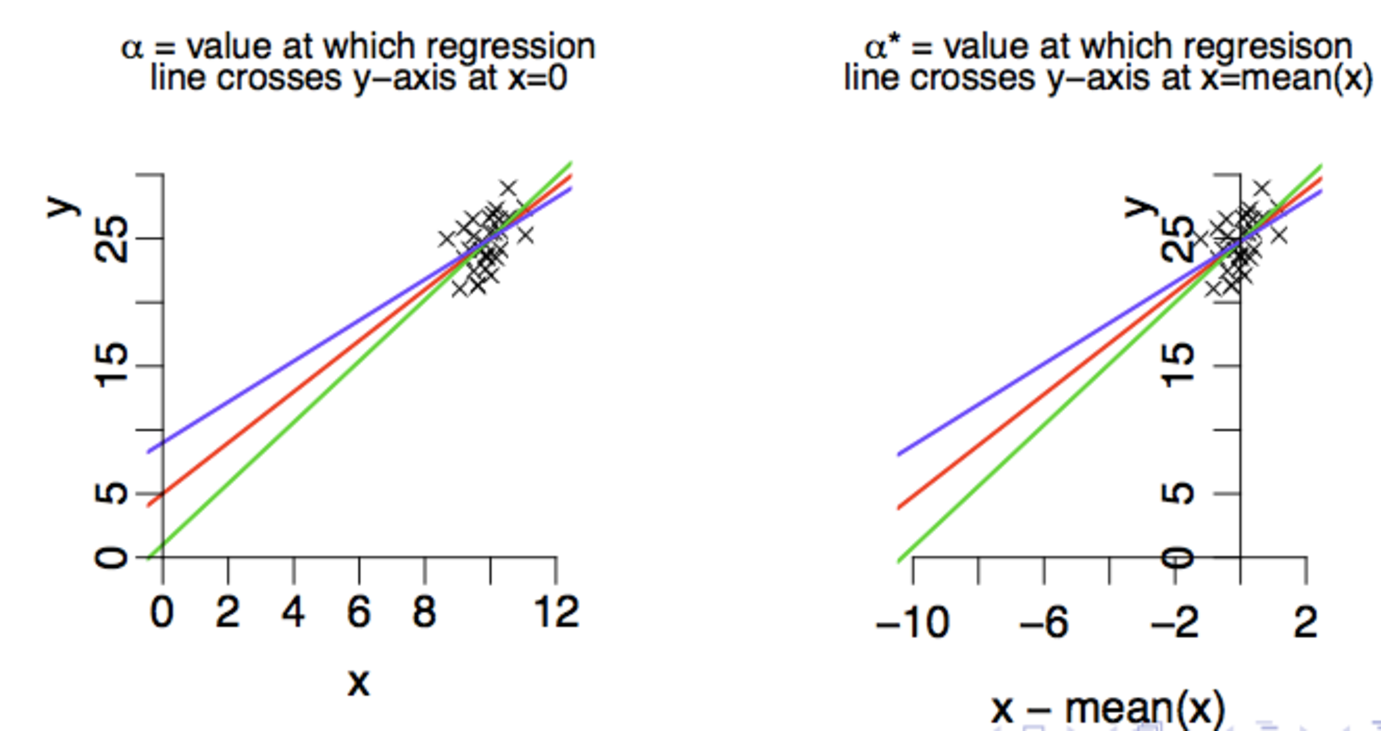
\includegraphics{Figures/covariate-centering.pdf}}
\end{center}
\end{frame}

\begin{frame}[fragile]
\frametitle{Output for \lq centred' analysis}
\begin{center}
\scalebox{0.38}{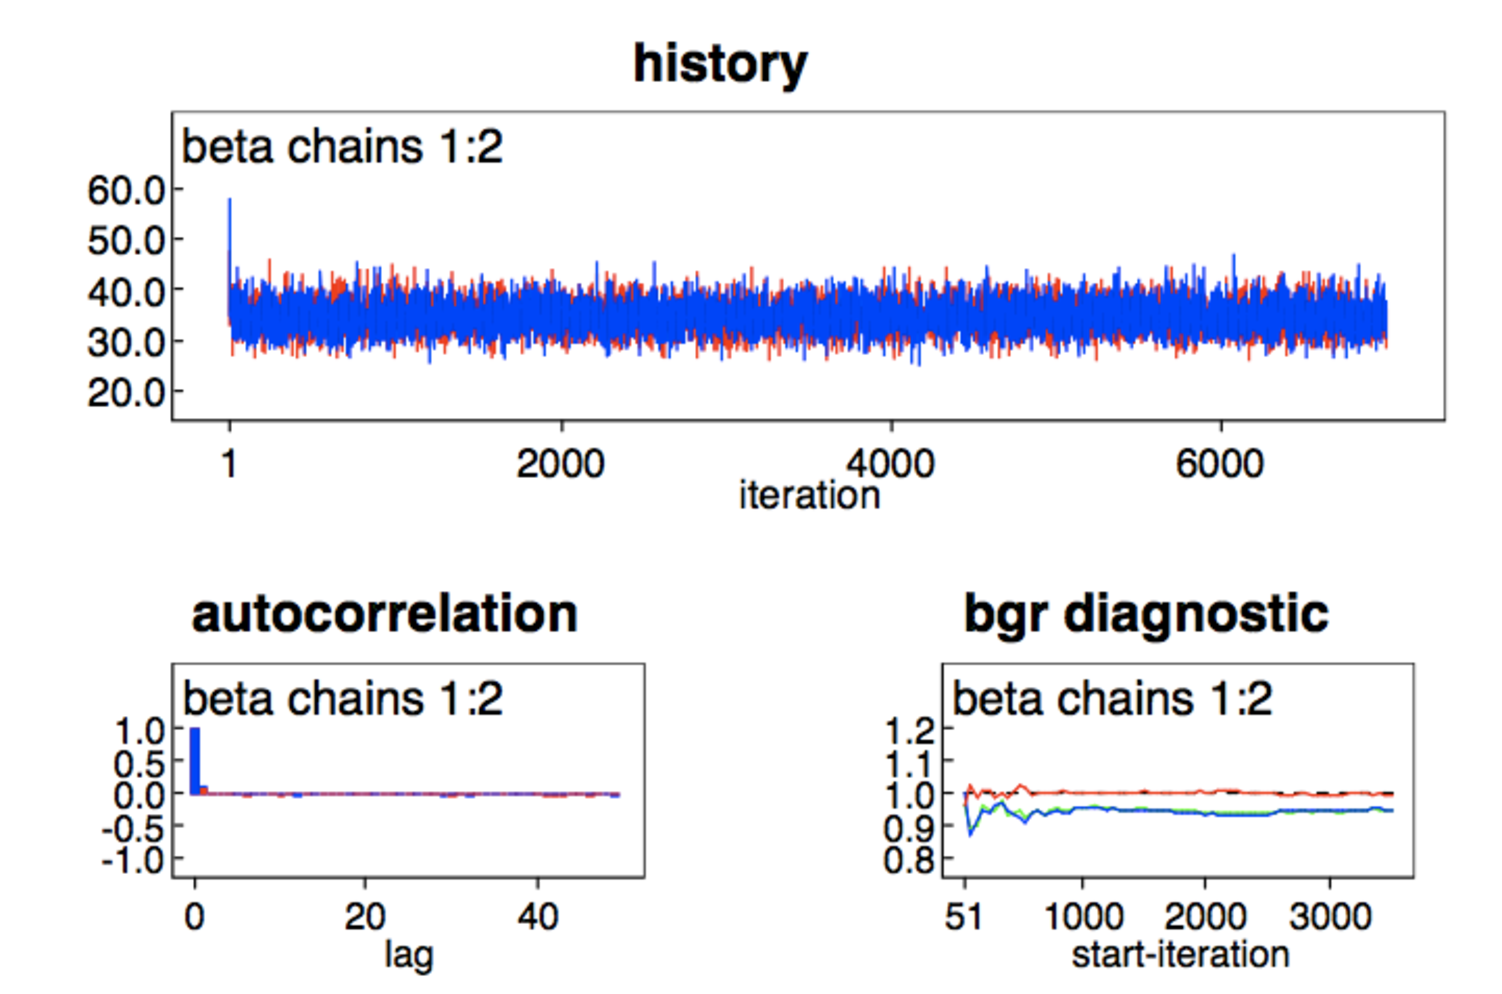
\includegraphics{Figures/dose-centered-out-2009.pdf}}
\end{center}
Discard first 1,000 iterations as burn-in
\begin{footnotesize}
\begin{verbatim}
node  mean  sd    MC error 2.5%   median  97.5%  start sample
beta  34.6  2.93  0.0298   29.17  34.54   40.6   1001  12000
\end{verbatim}
\end{footnotesize}
\end{frame}

\begin{frame}
\frametitle{OpenBUGS steps}
 \bi
 \I Load data files\vspace{2mm}
 \I Load multiple initial values files\vspace{2mm}
 \I Visually inspect trace plots\vspace{2mm}
 \I Check bgr diagnostics\vspace{2mm}
 \I Check autocorrelation plots\vspace{2mm}
 \I Discard burn-in samples\vspace{2mm}
 \ei
\end{frame}


\begin{frame}
\frametitle{How many iterations after convergence?}
\bibig
\item After convergence, further iterations are needed to obtain samples for posterior inference\vspace{2mm}
\item More iterations = more accurate posterior estimates\vspace{2mm}
%\item Rule of thumb: for well-behaved posterior, 95\% interval based on 4000 \alert{independent} samples will have actual posterior
%      probability between 94\% and 96\% (Raftery and Lewis, 1992)\vspace{2mm}
\item MCMC samples are usually \alert{autocorrelated} so effective sample size < actual sample size
\eibig
\end{frame}


\begin{frame}
\frametitle{Effective sample size and MC error}
\bibig
\I  Monte Carlo standard error (MCSE) = standard error of the mean of the posterior samples of $\theta$ as estimate of
      theoretical posterior expectation, $\E(\theta |y)$\vspace{2mm}
\I With independent samples, MCSE$^{ind}$ = $s / \sqrt{N}$,
where $s$ = posterior SD of $\theta$ and $N$ = sample size\vspace{2mm}
\I With autocorrelated samples, calculation of MCSE$^{ac}$ also depends on the autocorrelation\\\vspace{1mm}
$\rightarrow$ MCSE$^{ac}$ $>$ MCSE$^{ind}$\vspace{2mm}
\I An estimate of the \alert{effective sample size}, $N^*$ of an autocorrelated chain can be obtained as
$$N^* = (s/\hbox{MCSE}^{ac})^2$$\vspace{-3mm}
   \bibig
   \I so, if MCSE$^{ac} \approx 0.05 s \Rightarrow N^* \approx 1/0.05^2 = 400$\vspace{1mm}
   \I so, if MCSE$^{ac} \approx 0.015 s \Rightarrow N^* \approx 1/0.015^2 = 4444$\vspace{1mm}
   \I so, if MCSE$^{ac} \approx 0.01 s \Rightarrow N^* \approx 1/0.01^2 = 10000$
   \eibig
\eibig

\end{frame}

\begin{frame}[fragile]
\frametitle{Deciding if your posterior sample size is large enough}
\bibig
\I Relationship between posterior SD and MC error (previous slide) implies general rule for determining posterior sample size\vspace{1mm}
\bibig
\I after convergence, run MCMC simulation until the MC error $\approx$ 2 orders of magnitude smaller than the posterior SD\vspace{1mm}
\I[$\Rightarrow$] posterior summaries will be based on effective sample size of $\approx$10,000\vspace{2mm}
\eibig
\eibig
Output from logistic regression model with uncentred covariate\vspace{-2mm}
\begin{footnotesize}
\begin{verbatim}
node  mean   sd    MC error 2.5%   median  97.5%  start sample
beta  33.36  3.00  0.2117   28.18  33.5    38.33  10001 20000
\end{verbatim}\vspace{-2mm}
(MC error)/(sd) = 0.2117/3.00 = 0.07, so effective sample size $\approx 1/0.07^2$ = 204
\end{footnotesize}

\vspace{0.4cm}

Output from logistic regression model with centered covariate\vspace{-2mm}
\begin{footnotesize}
\begin{verbatim}
node  mean  sd    MC error 2.5%   median  97.5%  start sample
beta  34.6  2.93  0.0298   29.17  34.54   40.6   1001  12000
\end{verbatim}\vspace{-2mm}
(MC error)/(sd) = 0.0298/2.93 = 0.01, so effective sample size $\approx 1/0.01^2$ = 10,000
\end{footnotesize}

\end{frame}

\begin{frame}[t]

\frametitle{Key References and Further Reading}

%\begin{footnotesize}

Brooks, SP (1998). Markov chain Monte Carlo method and its
application. {\it The Statistician}, {\bf 47}, 69-100. \\ \vspace{2mm}

Brooks, SP and Gelman, A (1998). Alternative methods for
monitoring convergence of iterative simulations. {\it Journal of
Computational and Graphical Statistics}, {\bf 7}, 434-455. \\ \vspace{2mm}

Casella, G  and George, EI (1992). Explaining the Gibbs sampler.
{\it The American Statistician}, {\bf 46}, 167--174. \\ \vspace{2mm}

Cowles, MK and Carlin, BP (1996) Markov chain Monte Carlo
convergence diagnostics: a comparative review. {\it Journal of the
American Statistical Association}, {\bf 91}, 883--904. \\ \vspace{2mm}

Spiegelhalter, DJ, Gilks, WR and Richardson, S (1996). {\it Markov
chain Monte Carlo in Practice}, Chapman \& Hall, London. \\ %\vspace{2mm}

%\end{footnotesize}

\end{frame}
